\documentclass[aspectratio=169,serif]{beamer}
\usepackage{pifont}% http://ctan.org/pkg/pifont
\newcommand{\cmark}{\ding{51}}%
\newcommand{\xmark}{\ding{55}}
%\usetheme{SimplePlus}
\usetheme{Madrid}
%\usepackage[all]{xy}

%% packages
\usepackage{graphics,color,subfigure,pgf}
\usepackage{times,amsmath,amsbsy,amssymb,amscd,mathrsfs,chemarrow}
\usepackage{wasysym,mathtools}
\usepackage{multimedia}
\usepackage{hyperref}
\usepackage{booktabs} % Allows the use of \toprule, \midrule and \bottomrule in 
\usepackage{tikz,tikz-cd}

%% color
\usecolortheme{default}
%\newcommand{\red}[1]{\textcolor{red}{#1}}
%\newcommand{\blue}[1]{\structure{#1}}
%\newcommand{\brown}[1]{\textcolor{brown}{#1}}
%\newcommand{\green}[1]{\textcolor{green}{#1}}
\newcommand{\cyan}[1]{\textcolor{cyan}{#1}}
\newcommand{\red}[1]{\textcolor{red!75}{#1}}
\newcommand{\blue}[1]{\textcolor{blue!75}{#1}}
\newcommand{\brown}[1]{\textcolor{brown}{#1}}
\definecolor{darkgreen}{rgb}{0.1,0.65,0.1}
\newcommand{\green}[1]{\textcolor{darkgreen}{#1}}
\setbeamercolor{block title}{bg=black!80,fg = brown!90}

%% figure
\usepackage{tikz}
\usetikzlibrary{snakes}
\usetikzlibrary{arrows}
\usetikzlibrary{shapes}

%% diagram
\usepackage{stmaryrd}
\usepackage{chemarrow}
\usetikzlibrary{arrows}
\usepackage{multirow}

%% math operators
\renewcommand{\div}{\operatorname{div}}
\DeclareMathOperator*{\curl}{curl}
\DeclareMathOperator*{\grad}{grad}
\DeclareMathOperator*{\rot}{rot}
\DeclareMathOperator*{\range}{range}
\DeclareMathOperator*{\img}{img}
\newcommand{\tr}{\textrm{tr}}
\DeclareMathOperator*{\var}{Var}


%% shortcut
\newcommand{\bs}{\boldsymbol}
\newcommand{\mcal}{\mathcal}
\newcommand{\dx}{\,{\rm d}x}
\newcommand{\dd}{\,{\rm d}}


%% theorems
\newtheorem{remark}[theorem]{Remark}
\setcounter{tocdepth}{1} 
%\newtheorem{remark}{Remark}[section]
\setbeamertemplate{theorems}[numbered]
\setbeamertemplate{caption}[numbered]

\newcommand{\step}[1]{\noindent\raisebox{1.5pt}[10pt][0pt]{\tiny\framebox{$#1$}}\xspace}










\usepackage{algorithm2e}
\usepackage{stmaryrd}
\usepackage{chemarrow}
\usepackage[all]{xy}
\definecolor{darkgreen}{rgb}{0.1,0.65,0.1}
%\setbeamertemplate{blocks}[rounded][shadow=true]
%\setbeamercolor{block body}{fg=black,bg=darkgreen!15}
\setbeamercolor{block title}{bg=black!20,fg = black!90!cyan}

\usepackage{bookmark}
\hypersetup{bookmarksdepth=4,bookmarksnumbered=true,bookmarksopen=true}
\setbeamertemplate{footline}[frame number]
\setbeamertemplate{navigation symbols}{}

\newcommand{\dev}{\operatorname{dev}}
\newcommand{\sym}{\operatorname{sym}}
\newcommand{\skw}{\operatorname{skw}}
\newcommand{\spn}{\operatorname{spn}}
\newcommand{\defm}{\operatorname{def}}
\newcommand{\sign}{\operatorname{sign}}
\newcommand{\hess}{\operatorname{hess}}
\newcommand{\inc}{\operatorname{inc}}
\newcommand{\Oplus}{\ensuremath{\vcenter{\hbox{\scalebox{1.5}{$\oplus$}}}}}
\DeclareMathOperator*{\spa}{span}
\newcommand{\dist}{\operatorname{dist}}

%\DeclareMathOperator*{\curl}{curl}
% \DeclareMathOperator*{\img}{img}
% \DeclareMathOperator*{\spa}{span}
\DeclareMathOperator*{\diag}{diag}
% \newcommand{\curl}{{\rm curl\,}}
\renewcommand{\div}{\operatorname{div}}
%\renewcommand{\grad}{\operatorname{grad}}
% \newcommand{\grad}{{\rm grad\,}}
%\DeclareMathOperator*{\tr}{tr}
% \DeclareMathOperator*{\rot}{rot}
% \DeclareMathOperator*{\var}{Var}
\DeclareMathOperator{\rank}{rank}
% \DeclareMathOperator{\dist}{dist}
%\DeclareMathOperator{\span}{span}
% \newcommand{\tr}{\operatorname{tr}}
% \newcommand{\dev}{\operatorname{dev}}
% \newcommand{\sym}{\operatorname{sym}}
% \newcommand{\skw}{\operatorname{skw}}
% \newcommand{\spn}{\operatorname{spn}}
\newcommand{\mspn}{\operatorname{mspn}}
\newcommand{\vspn}{\operatorname{vspn}}
\newcommand{\mskw}{\operatorname{mskw}}
\newcommand{\vskw}{\operatorname{vskw}}
% \newcommand{\defm}{\operatorname{def}}
% \newcommand{\hess}{\operatorname{hess}}
% \newcommand{\inc}{\operatorname{inc}}
\newcommand{\dex}{\operatorname{dex}}

% \usepackage{fontspec}
%\setCJKmainfont{Songti SC Regular}
%\setmainfont{Kaiti SC Regular}
% \setsansfont{Songti SC Regular}
% \setmainfont{Times New Roman}

\usepackage{xeCJK}

\newcommand{\kai}{\CJKfontspec{Kaiti SC}}



%\usebackgroundtemplate{\includegraphics[width=4.5in]{figures/UCIwatermark1.png}}

\begin{document}

\title{新型虚单元方法的理论,实现及应用研究}
\author{陈春雨}
\institute[XTU]{
导师:魏华祎\\
    cbtxs@smail.xtu.edu.cn\\
\vspace{5pt}
湘潭大学\\
数学与计算科学学院
}
 
\date
{
    \today
}

\pgfdeclareimage[height=1cm]{institution-logo}{../figures/xtu.pdf}

\logo{\pgfuseimage{institution-logo}}

\frame[plain]{\titlepage}

\AtBeginSection[]{

  \frame<beamer>{ 

    \frametitle{Outline}   

    \tableofcontents[currentsection] 
  }
}
\section{虚单元方法简介}
\begin{frame}
  \frametitle{Poisson 方程的虚单元方法}

  Poisson 方程的虚单元方法为:找到 $u_h \in V_h$,满足:
  $$
  a_h(u_h, v_h) = (f, v_h), \quad \forall v_h \in V_h,
  $$
  其中:
  $$
  a_h(u_h, v_h) = \sum_{K \in \mathcal{T}_h} a_h^K(u_h, v_h),
  $$


\end{frame}



\section{理论篇}
\subsection{二阶椭圆方程的虚单元方法}
\begin{frame}
  \frametitle{一般椭圆方程}
\end{frame}

\begin{frame}
  \frametitle{$H^1$ 协调的虚单元空间}
\end{frame}

\begin{frame}
  \frametitle{$H^1$ 非协调的虚单元空间}
\end{frame}

\begin{frame}
  \frametitle{无稳定子虚单元方法}
\end{frame}

\subsection{时谐 Maxwell 方程的虚单元方法}

\subsubsection{各向异性界面问题的虚单元方法}

\subsection{高阶椭圆方程的虚单元方法求解}

\section{实现篇}
\subsection{网格}
\begin{frame}    
    \frametitle{Halfedge Mesh}
\end{frame}

\begin{frame}    
    \frametitle{Dart Mesh}
\end{frame}


\subsection{空间}
\begin{frame}
\frametitle{Scaled monomial space}
\begin{minipage}[b]{0.55\linewidth}
对于 $\boldsymbol{\alpha} = (\alpha_0, \alpha_1) \in \mathbb{T}_1^k$, 
定义 $K$ 上的缩放单项式:
$$
m_{\boldsymbol{\alpha}}(\boldsymbol{x}) = \frac{(\boldsymbol{x} - \boldsymbol{x}_K)^{\alpha_0}(y -
y_K)^{\alpha_1}}{h_K^{|\boldsymbol{\alpha}|}}
$$
其中:
\begin{itemize}
    \item $h_K$ 是 $K$ 的直径; 
    \item $\boldsymbol{x}_K = (x_K, y_K)$ 是 $K$ 的质心;
\end{itemize}
$\mathcal{M}_k = [m_0, m_1, m_2, \cdots, m_{n_k-1}], $
形成了 $\mathbb{P}_k(K)$ 的一组基。
\end{minipage}
\hfill
\begin{minipage}[b]{0.4\linewidth}
    \centering
    \begin{figure}[htpb]
        \centering
        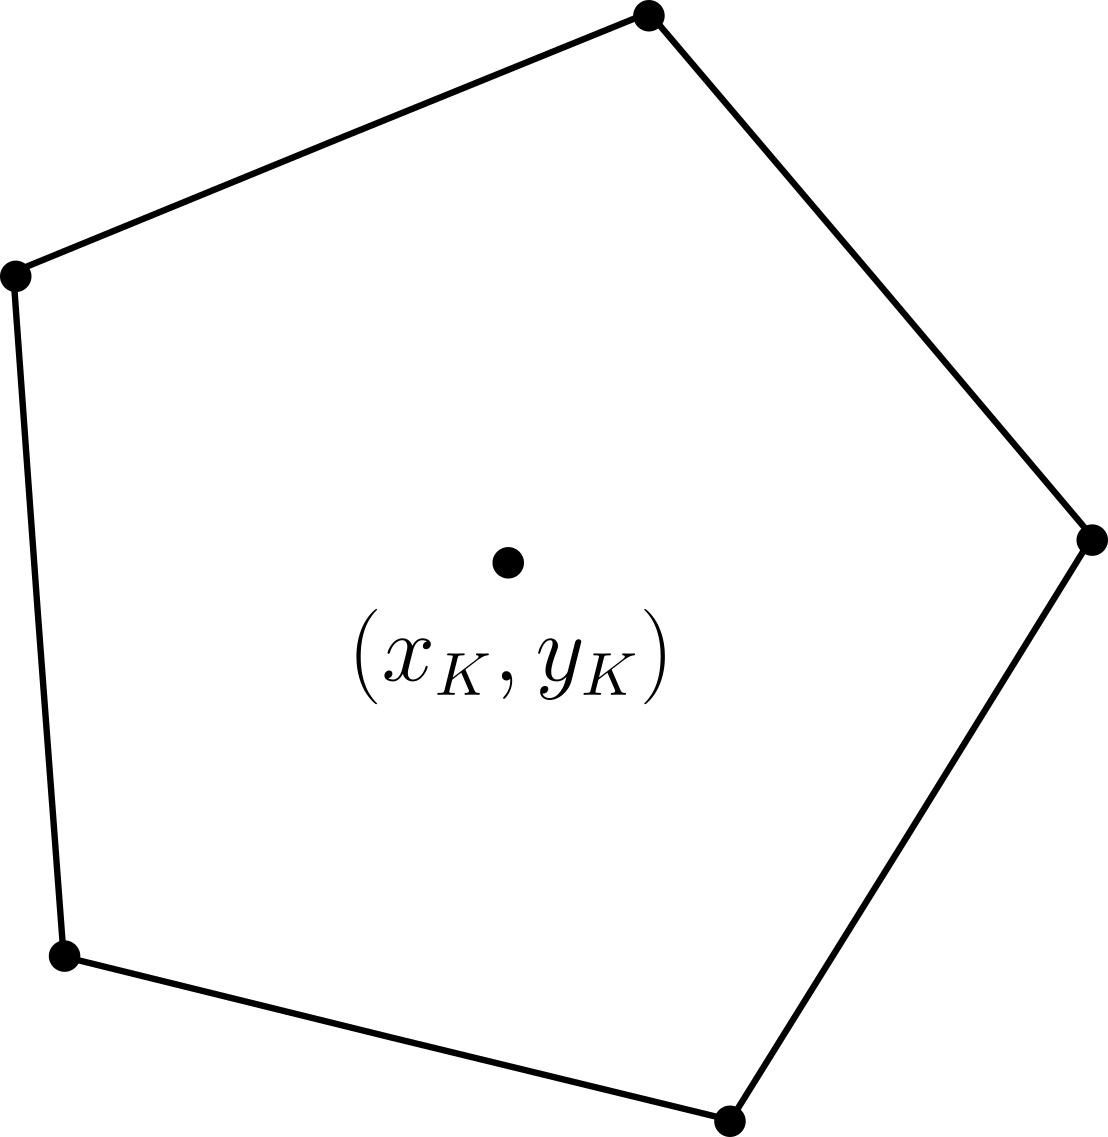
\includegraphics[width=0.8\textwidth]{../figures/polygon_K.png}
        \caption{Barycenter of $K$.}
    \end{figure}
\end{minipage}
\end{frame}

\begin{frame}
  \frametitle{Integration}
\end{frame}

\begin{frame}
  \frametitle{$H^1$ 协调的虚单元空间}
\end{frame}

\begin{frame}
  \frametitle{$H^1$ 非协调的虚单元空间}
\end{frame}

\begin{frame}
  \frametitle{无稳定子的虚单元空间}
\end{frame}

\begin{frame}
    \frametitle{$H(\mathrm{curl})$ 协调的虚单元空间}
\end{frame}

\begin{frame}
    \frametitle{$H^m$ 协调的虚单元空间}
\end{frame}

\subsection{数值算例}

\section{应用篇}

\subsection{超弹性问题的无稳定子虚单元方法}

\subsection{电磁界面问题的时域虚单元方法}

\end{document}
